\subsection{Другие объекты}

\subsubsection*{Рассеянное звёздное скопление}
\begin{wrapfigure}[7]{r}{0.32\tw}
    \vspace{-1pc}
    \centering
    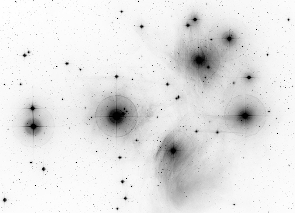
\includegraphics[width = 0.25\tw]{m45.pdf}
    \caption{Рассеянное звёздное скопление M45 (негатив)}
\end{wrapfigure}
Слабо связанная группа из сотен или тысяч звёзд, сформировавшихся из одного гигантского \imp{молекулярного облака} и имеющих одинаковый возраст. Рассеянные звёздные скопления встречаются только в тонком диске Галактики, их типичный диаметр~--- несколько парсек.
\begin{figure}[h!]
    \begin{subcaptionblock}{0.48\tw}
        \centering
        \tikzsetnextfilename{hr-m45}
        \begin{tikzpicture}
            \begin{axis}[
                height = 4.5cm,
                width  = 1.05\tw,
                xlabel = {$B-V$},
                ylabel = {$M_V$},
                ymax   = 8.0,
                ymin   = -2.0,
                y dir  = reverse,
                xmax   = 1.5,
                xmin   = -0.25
            ]
                \addplot+[only marks, mark = o, mark options={scale=0.2, black}] table[x=B-V, y=M_V]{data/hr-M45.txt};
            \end{axis}
        \end{tikzpicture}
        \caption{Диаграмма Герцшпрунга--Рассела скопления M45 (Плеяды)}
    \end{subcaptionblock}
    \hfill
    \begin{subcaptionblock}{0.48\tw}
        \centering
        \tikzsetnextfilename{hr-m67}
        \begin{tikzpicture}
            \begin{axis}[
                height = 4.5cm,
                width  = 1.05\tw,
                xlabel = {$B-V$},
                ylabel = {$M_V$},
                ymax   = 10.0,
                ymin   = 0.0,
                y dir  = reverse,
                xmax   = 1.5,
                xmin   = 0.25
            ]
                \addplot+[only marks, mark = o, mark options={scale=0.2, black}] table[x=B-V, y=M_V]{data/hr-M67.txt};
            \end{axis}
        \end{tikzpicture}
        \caption{Диаграмма Герцшпрунга--Рассела скопления M67}
    \end{subcaptionblock}
    \caption{}
\end{figure}

\subsubsection*{Шаровое звёздное скопление}
\begin{wrapfigure}[7]{r}{0.32\tw}
    \vspace{-1pc}
    \centering
    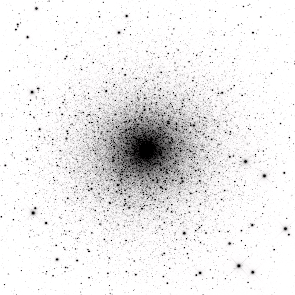
\includegraphics[width = 0.25\tw]{m13.pdf}
    \caption{Шаровое скопление M13 (негатив)}
\end{wrapfigure}
Скопление звёзд, состоящее из нескольких сотен тысяч светил, тесно связанных гравитацией. Млечный путь насчитывает около 160 шаровых звёздных скоплений. Диаметры шаровых скоплений составляют 20\,--\,60~пк, массы~--- $10^4$\,--\,$10^6$~солнечных.

\begin{figure}[h!]
    \begin{subcaptionblock}{0.48\tw}
        \centering
        \tikzsetnextfilename{hr-47-Tuc}
        \begin{tikzpicture}
            \begin{axis}[
                height = 4.5cm,
                width  = 1.05\tw,
                xlabel = {$B-V$},
                ylabel = {$M_V$},
                ymax   = 6.0,
                ymin   = -2.0,
                y dir  = reverse,
                xmax   = 1.75,
                xmin   = 0.25
            ]
                \addplot+[only marks, mark = o, mark options={scale=0.2, black}] table[x=B-V, y=M_V]{data/hr-47-Tuc.txt};
            \end{axis}
        \end{tikzpicture}
        \caption{Диаграмма Герцшпрунга--Рассела скопления 47\,Tuc}
    \end{subcaptionblock}
    \hfill
    \begin{subcaptionblock}{0.48\tw}
        \centering
        \tikzsetnextfilename{hr-m13}
        \begin{tikzpicture}
            \begin{axis}[
                height = 4.5cm,
                width  = 1.05\tw,
                xlabel = {$B-V$},
                ylabel = {$M_V$},
                ymax   = 8.0,
                ymin   = -2.0,
                y dir  = reverse,
                xmax   = 1.25,
                xmin   = -0.25
            ]
                \addplot+[only marks, mark = o, mark options={scale=0.2, black}] table[x=B-V, y=M_V]{data/hr-M13.txt};
            \end{axis}
        \end{tikzpicture}
        \caption{Диаграмма Герцшпрунга--Рассела скопления M13}
    \end{subcaptionblock}
    \caption{}
\end{figure}

\begin{wrapfigure}[7]{r}{0.32\tw}
    \vspace{-1pc}
    \centering
    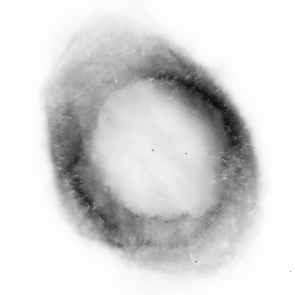
\includegraphics[width = 0.25\tw]{m57.pdf}
    \caption{Пла\-не\-тар\-ная туманность M57 (негатив)}
\end{wrapfigure}
\subsubsection*{Планетарная туманность}
 Система из звезды, называемой ядром туманности, и симметрично окружающей ее светящейся газовой оболочки. Планетарные туманности образуются при сбросе внешних слоёв (оболочек) красных гигантов и сверхгигантов с массой от $0.8M_\odot$ до $8M_\odot$ на завершающей стадии их эволюции. Характерный размер~--- 1\,--\,2~св.\,лет.
